\subsection{Comparison of CV models}
\label{sxn:cv}

Each of the VGG, ResNet, and DenseNet series of models consists of several pretrained DNN models, trained on the full ImageNet~\cite{imagenet} dataset, and each is distributed with the current open source pyTorch framework (version 1.4)~\cite{pytorch}.
In addition, we examine a larger set of ResNet models, which we call the ResNet-1K series, trained on the ImageNet-1K dataset~\cite{imagenet} and provided on the OSMR Sandbox~\cite{osmr}.
For these models, we first perform coarse model analysis, comparing and contrasting the four model series, and predicting trends in model quality.
We then perform fine layer analysis, as a function of depth.
This layer analysis goes beyond predicting trends in model quality, instead illustrating that PL-based metrics can provide novel insights among the VGG, ResNet/ResNet-1K, and DenseNet architectures. 


\paragraph{Average Quality Metrics versus Reported Test Accuracies.}

We examine the performance of the four quality metrics (Log Frobenius norm, Log Spectral norm, Weighted Alpha, and Log $\alpha$-Norm) applied to each of the VGG, ResNet, ResNet-1K, and DenseNet series.
Figure~\ref{fig:vgg-metrics} 
plots the four quality metrics versus reported test accuracies~\cite{pytorch},% 
\footnote{These test accuracies have been previously reported and made publicly-available by others.  We take them as given.  We do not attempt to reproduce/verify them, since we do not permit ourselves access to training/test data.}
as well as a basic linear regression line, for the VGG series.
All four metrics correlate quite well with reported Top1 accuracies, with smaller norms and smaller values of $\hat{\alpha}$ implying better generalization (i.e., greater accuracy, lower error). 
The Log $\alpha$-Norm metric ($\log\Vert\mathbf{W}\Vert_{\alpha}^{\alpha}$) performs best (RMSE of $0.42$, see Table~\ref{table:cv-models}); and the Weighted Alpha metric ($\hat\alpha =\alpha\log\lambda_{max} $) performs second best (RMSE of $0.48$, see Table~\ref{table:cv-models}).


\begin{figure}[t]
    \centering
    \subfigure[Log Frobenius Norm, VGG ]{
        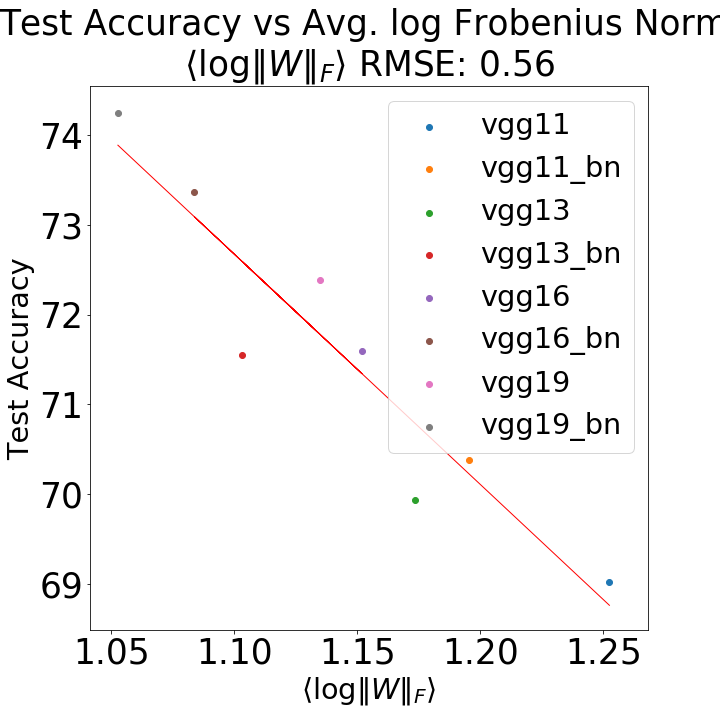
\includegraphics[width=4.9cm]{img/VGG_lognorm_accs.png}
        \label{fig:vgg-fnorm}
    }
    \qquad
    \subfigure[Log Spectral Norm, VGG ]{
        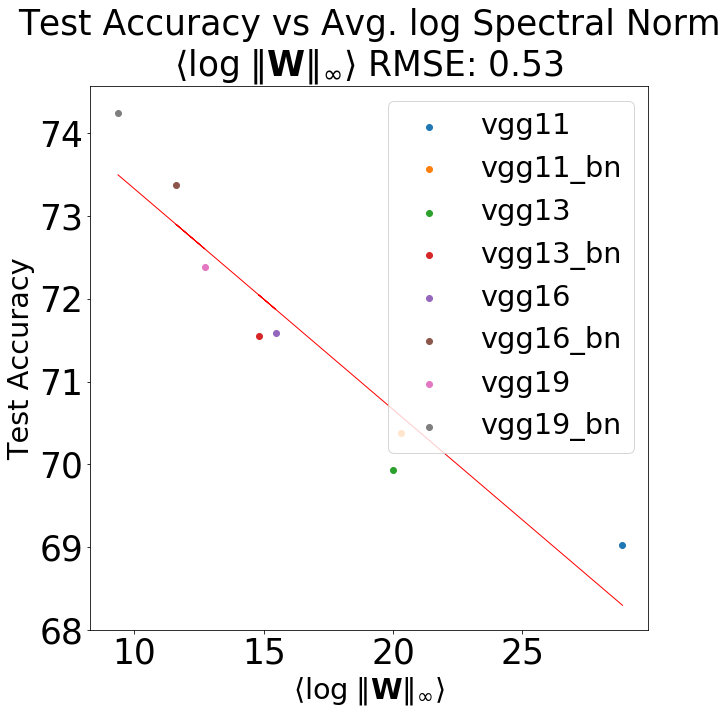
\includegraphics[width=4.9cm]{img/VGG_spectralnorm_accs.png}
        \label{fig:vgg-snorm}
    }
    \qquad
    \subfigure[ Weighted Alpha, VGG ]{
        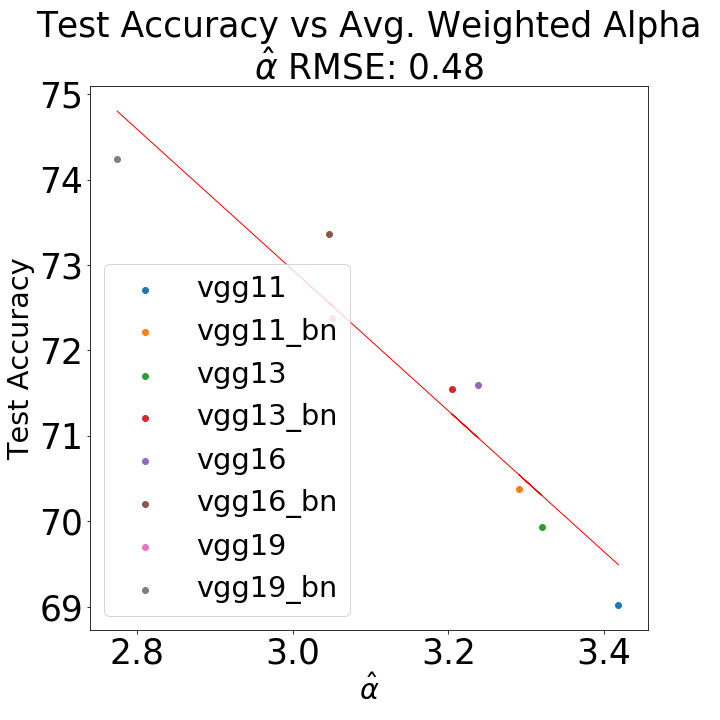
\includegraphics[width=4.9cm]{img/VGG_alpha_weighted_accs.png}
        \label{fig:vgg-walpha}
    }
    \qquad
    \subfigure[Log $\alpha$-Norm, VGG ]{
        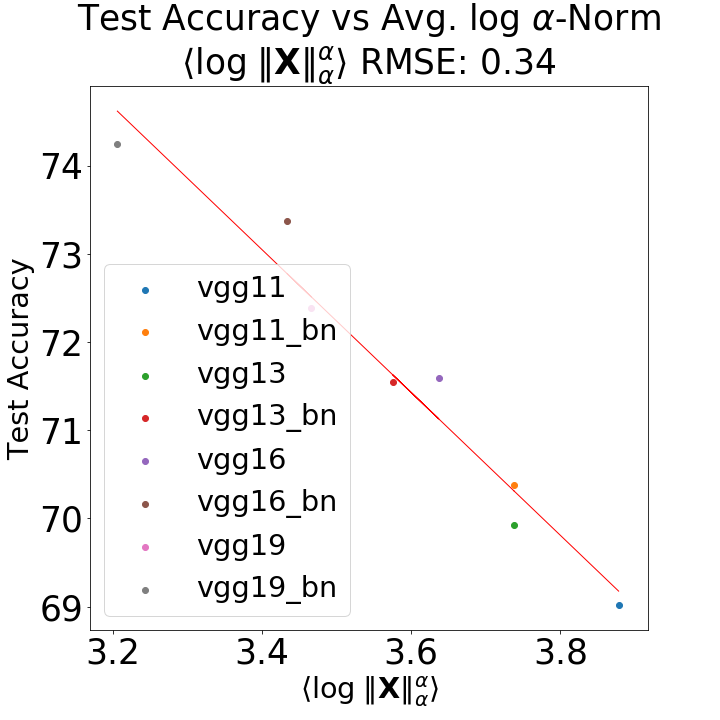
\includegraphics[width=4.9cm]{img/VGG_logpnorm_accs.png}
        \label{fig:vgg-pnorm}
    }
    \caption{Comparison of Average Log Norm and Weighted Alpha quality metrics versus reported test accuracy for pretrained VGG models: 
             VGG11, VGG13, VGG16, and VGG19, with and without Batch Normalization (BN),
             trained on ImageNet, available in pyTorch (v1.4).  
             Metrics fit by linear regression, RMSE reported.  }
    \label{fig:vgg-metrics}
\end{figure}


\begin{figure}[t]
    \centering

    \subfigure[ ResNet, Log $\alpha$-Norm ]{
        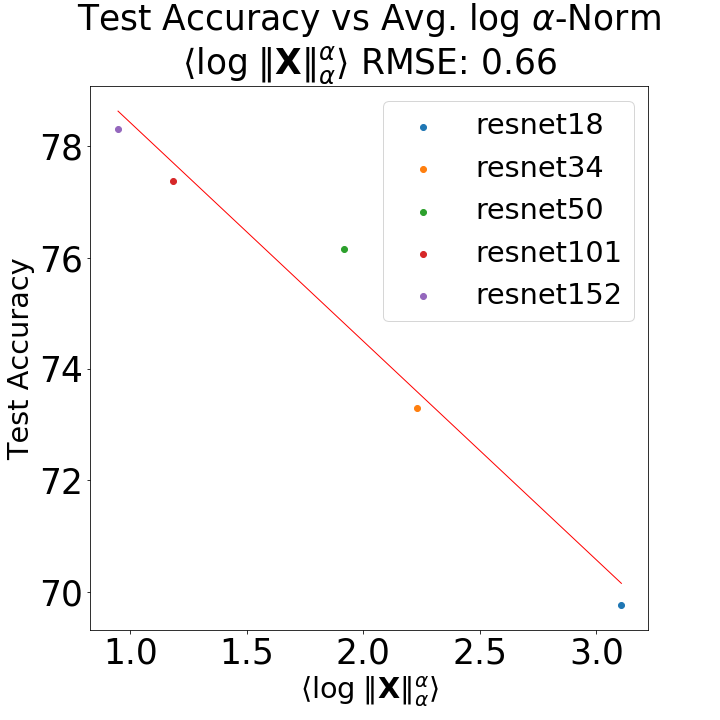
\includegraphics[width=4.9cm]{img/ResNet_logpnorm_accs.png}
        \label{fig:resnet-accuracy}
    }
    \qquad
    \subfigure[ ResNet-1K, Log $\alpha$-Norm ]{
        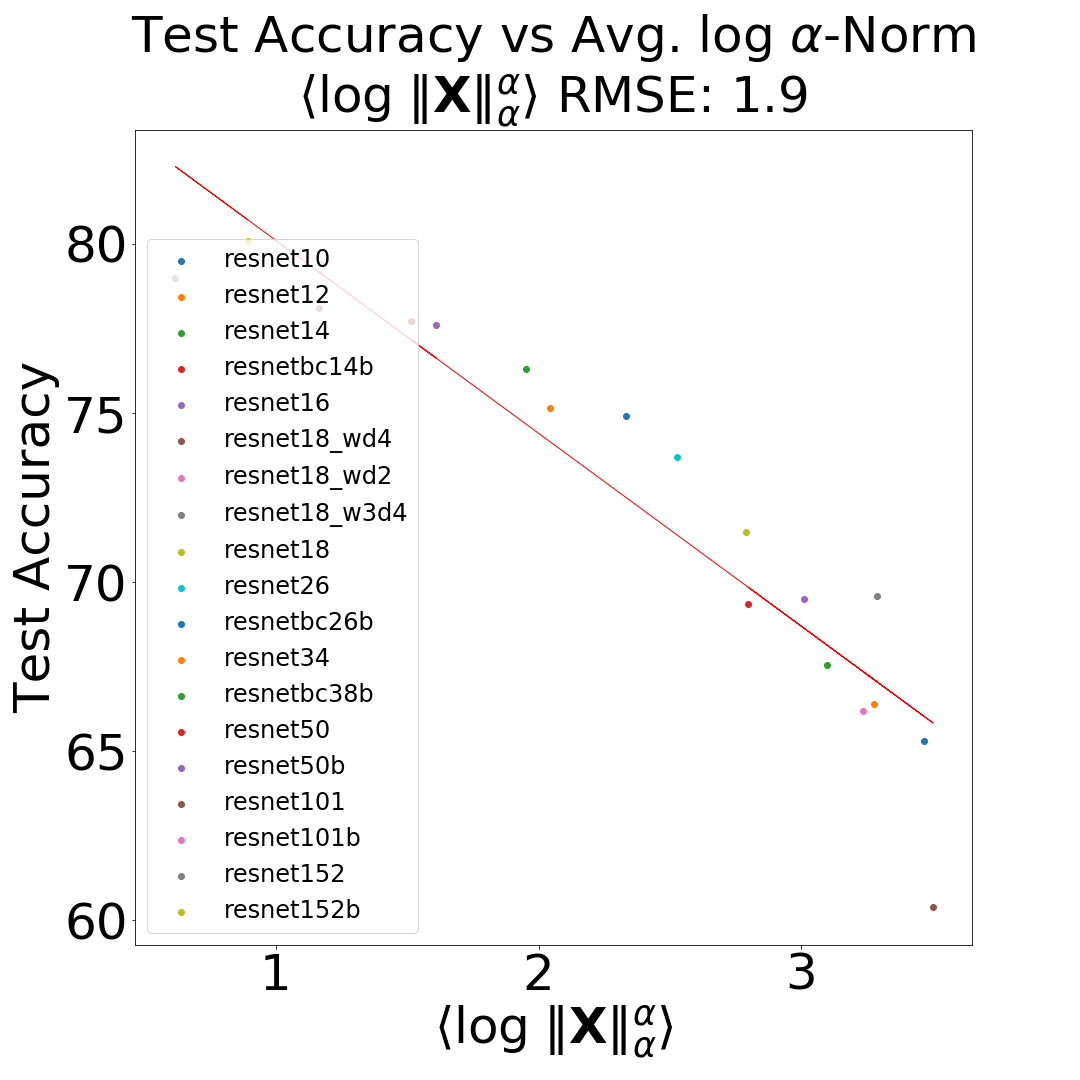
\includegraphics[width=4.9cm]{img/ResNet-1K_logpnorm_accs.png}
        \label{fig:resnet1k-accuracy}
    }
    \caption{Comparison of Average $\alpha$-Norm quality metric versus reported Top1 test accuracy for the ResNet and ResNet-1K pretrained (pyTorch) models. 
             \michael{Symbols and text are way to small on these and other figures; axes/ticks way too small; need different symbols, not just red versus green; etc.}
            }
    \label{fig:cv2-accuracy}
\end{figure}


\begin{table}[t]
\small
\begin{center}
\begin{tabular}{|p{1in}|c|c|c|c|c|}
\hline
 Series    &\#   & $\langle\log\Vert\mathbf{W}\Vert_{F}\rangle$ & $\langle\log\Vert\mathbf{W}\Vert_{\infty}\rangle$ & $\hat{\alpha}$ & $\langle\log\Vert\mathbf{X}\Vert^{\alpha}_{\alpha}\rangle$ \\
\hline
 VGG       &  6 & 0.56 & 0.53 & 0.48          & \textbf{0.42}  \\
 ResNet    &  5 & 0.9  & 1.4  & \textbf{0.61} & 0.66           \\
 ResNet-1K & 19 & 2.4  & 3.6  & \textbf{1.8}  & 1.9            \\
 DenseNet  &  4 & 0.3  & 0.26 & \textbf{0.16} & 0.21           \\
\hline
\end{tabular}
\end{center}
\caption{RMSE (smaller is better) for linear fits of 
         quality metrics to reported Top1 test error for pretrained models in each architecture series.  
         Column \# refers to number of models.  
         VGG, ResNet, and DenseNet were pretrained on ImageNet.  
         ResNet-1K was pretrained on ImageNet-1K. 
}
\label{table:cv-models}
\end{table}

See Table~\ref{table:cv-models} for a summary of results for Top1 accuracies for all four metrics for the VGG, ResNet, ResNet-1K, and DenseNet series.
Similar results (not shown) are obtained for the Top5 accuracies.
Overall, all metrics perform relatively well; the Weighted Alpha metric performs best; and the Log $\alpha$-Norm metric performs second best.
These model series are all very well-trodden, and our results indicate that norm-based metrics and PL-based metrics can both distinguish among a series of well-trained versus very-well-trained models, with PL-based metrics performing somewhat (i.e., quantitatively) better.
The DenseNet series has similar behavior.
(These and many other such plots can be seen on our publicly-available~repo.)


To examine how the four quality metrics depend on data set size, we look at results on ResNet versus ResNet-1K.
Figure~\ref{fig:cv2-accuracy} compares the Log $\alpha$-Norm metric for the full ResNet model, trained on the full ImageNet dataset, against the ResNet-1K model, trained on a much smaller ImageNet-1K data set.
The Log $\alpha$-Norm is much better than the Log Frobenius/Spectral norm metrics (although, as Table~\ref{table:cv-models} shows, it is slightly worse than the Weighted Alpha metric).
The ResNet series has strong correlation, with an RMSE of $0.66$, whereas the ResNet-1K series also shows good correlation, but has a much larger RMSE of $1.9$.
(Other metrics exhibit similar behavior.)
The higher quality data set shows a better fit, even with fewer data~points.


\paragraph{Layer Analysis: Metrics as a Function of Depth.}

We can learn much more about a pretrained model by going beyond average values of quality metrics to examining quality metrics for each layer weight matrix, $\mathbf{W}$, as a function of depth (or layer id).  
Figure~\ref{fig:3models-alpha-layers} plots the PL exponent $\alpha$, as a function of depth, for each layer (first layer corresponds to data, last layer to labels) for the least accurate (shallowest) and most accurate (deepest) model in each of the VGG (no BN), ResNet, and DenseNet series.
(Many more such plots are available at our repo.)

\begin{figure}[t]
    \centering

    \subfigure[ VGG ]{
        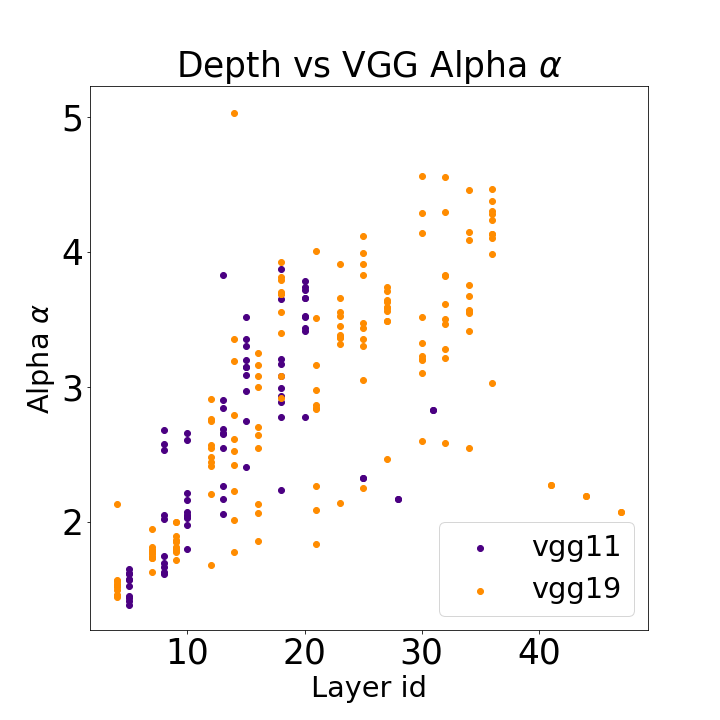
\includegraphics[width=4.9cm]{img/VGG_fnl_alpha_depth.png} 
                \label{fig:vgg-alpha-layers}
    }
    \qquad
    \subfigure[ ResNet ]{
        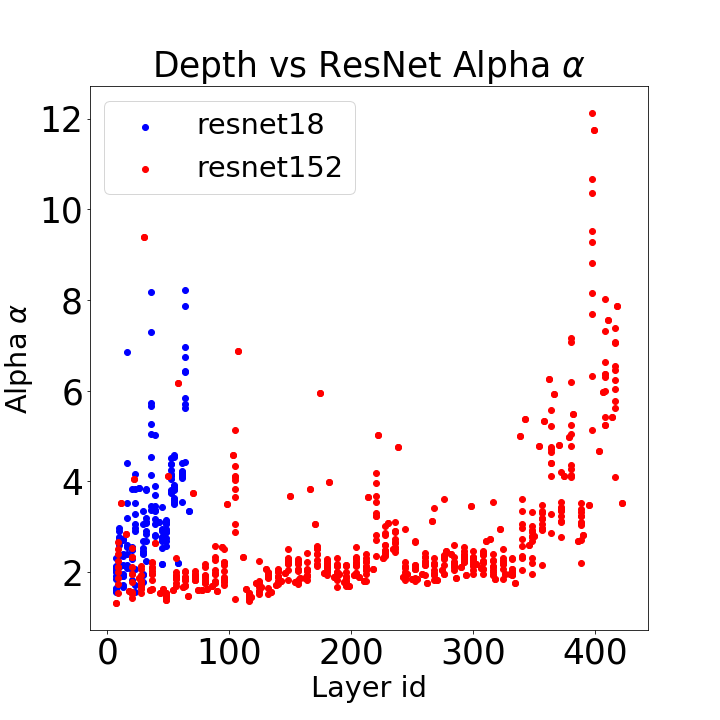
\includegraphics[width=4.9cm]{img/ResNet_fnl_alpha_depth.png} 
        \label{fig:resnet-alpha-layer}
    }
    \qquad
    \subfigure[ DenseNet ]{
        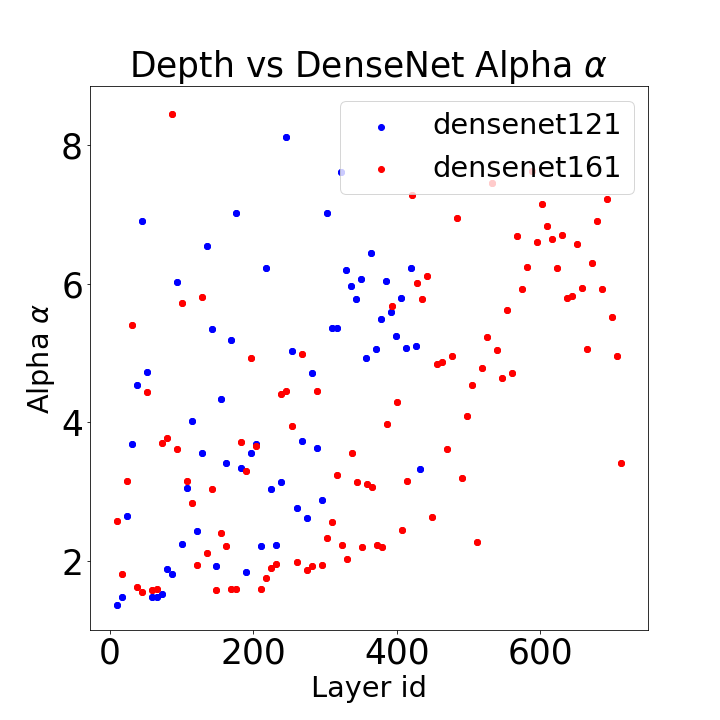
\includegraphics[width=4.9cm]{img/DenseNet_fnl_alpha_depth.png} 
        \label{fig:densenet-alpha-layer}
    }    
    \qquad
    \subfigure[ ResNet (overlaid) ]{
        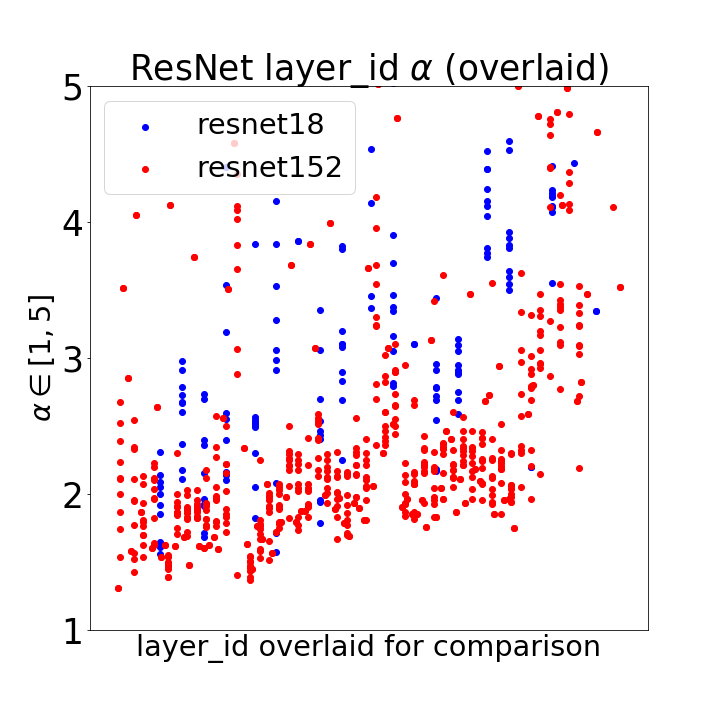
\includegraphics[width=4.9cm]{img/resnet_alpha_overlaid_depth.png} 
        \label{fig:resnet_alpha_overlaid_depth}
    }
    \caption{PL exponent ($\alpha$) versus layer id, for the least and the most accurate models in VGG (a), ResNet (b), and DenseNet (c) series. 
             (VGG is without BN; and note that the Y axes on each plot are different.)  
             Subfigure (d) displays the ResNet models (b), zoomed in to $\alpha\in[1,5]$, and with the layer ids overlaid on the X-axis, from smallest to largest, to
             allow a more detailed analysis of the most strongly correlated layers.
             Notice that ResNet152 exhibits different and much more stable behavior of $\alpha$ across layers.
             This contrasts with how both VGG models gradually worsen in deeper layers and how the DenseNet models are much more erratic.  
             In the text, this is interpreted in terms of Correlation Flow.
            }
    \label{fig:3models-alpha-layers}
\end{figure}

In the VGG models, Figure~\ref{fig:vgg-alpha-layers} shows that the PL exponent $\alpha$ systematically increases as we move down the network, from data to labels, in the Conv2D layers, starting with $\alpha\lesssim 2.0$ and reaching all the way to $\alpha\sim 5.0$; and then, in the last three, large, fully-connected (FC) layers, $\alpha$ stabilizes back down to $\alpha\in[2,2.5]$.
This is seen for all the VGG models (again, only the shallowest and deepest are shown), indicating that the main effect of increasing depth is to increase the range over which $\alpha$ increases, thus leading to larger $\alpha$ values in later Conv2D layers of the VGG models.
This is quite different than the behavior of either the ResNet-1K models or the DenseNet models.

For the ResNet-1K models, Figure~\ref{fig:resnet-alpha-layer} shows that $\alpha$ also increases in the last few layers (more dramatically than for VGG, observe the differing scales on the Y axes).
However, as the ResNet-1K models get deeper, there is a wide range over which $\alpha$ values tend to remain small.
This is seen for other models in the ResNet-1K series, but it is most pronounced for the larger ResNet-1K (152) model, where $\alpha$ remains relatively stable at $\alpha\sim 2.0$, from the earliest layers all the way until we reach close to the final layers.  

For the DenseNet models, Figure~\ref{fig:densenet-alpha-layer} shows that $\alpha$ tends to increase as the layer id increases, in particular for layers toward the end.
While this is similar to the VGG models, with the DenseNet models, $\alpha$ values increase almost immediately after the first few layers, and the variance is much larger (in particular for the earlier and middle layers, where it can range all the way to $\alpha\sim 8.0$) and much less systematic throughout the network.


\paragraph{Correlation Flow; or How $\alpha$ Varies Across Layers.}

Figure~\ref{fig:3models-alpha-layers} can be understood in terms of what we will call Correlation Flow.
The average Log $\alpha$-Norm metric and the Weighted Alpha metric are based on HT-SR Theory~\cite{MM18_TR, MM19_HTSR_ICML, MM20_SDM}, which is in turn based on the statistical mechanics of heavy tailed and strongly correlated systems~\cite{BouchaudPotters03, SornetteBook, BP11, bun2017}. 
There, one expects that the weight matrices of well-trained DNNs will exhibit correlations over many size scales, as is well-known in other strongly-correlated systems~\cite{BouchaudPotters03, SornetteBook}. 
This would imply that their ESDs can be well-fit by a truncated PL, with exponents $\alpha\in[2,4]$.
Much larger values $(\alpha\gg 6)$ may reflect poorer PL fits, whereas smaller values $(\alpha\sim 2)$, are associated with models that generalize better.

Informally, one would expect a DNN model to perform well when it facilitates the propagation of information/features across layers.
In the absence of training/test data, one might hypothesize that this flow of information leaves empirical signatures on weight matrices, and that we can quantify this by measuring the PL properties of weight matrices.
In this case, smaller $\alpha$ values correspond to layers in which information correlations between data across multiple scales are better captured~\cite{MM18_TR,SornetteBook}.
This leads to the hypothesis that small $\alpha$ values that are stable across multiple layers enable better correlation flow through the network.
This is similar to recent work on the information bottleneck~\cite{ST17_TR}, except that here we work in an entirely unsupervised setting.

\begin{figure}[t]
   \centering
   \subfigure[$\lambda_{max}$ for ResNet20 layers]{
      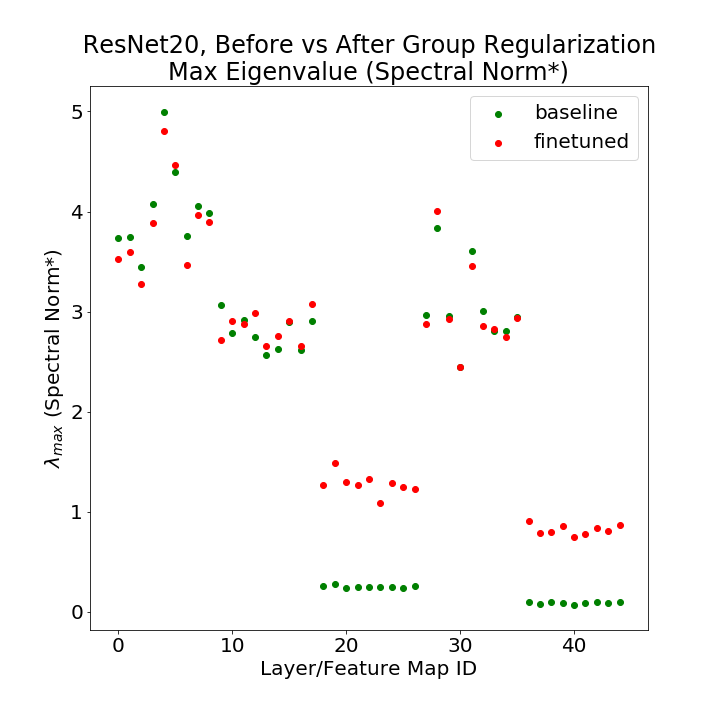
\includegraphics[width=4.9cm]{img/resnet4d_maxev.png}
      \label{fig:resnet204Dmaxev}
   }
   \qquad
   \subfigure[$\alpha$ for ResNet20 layers]{
      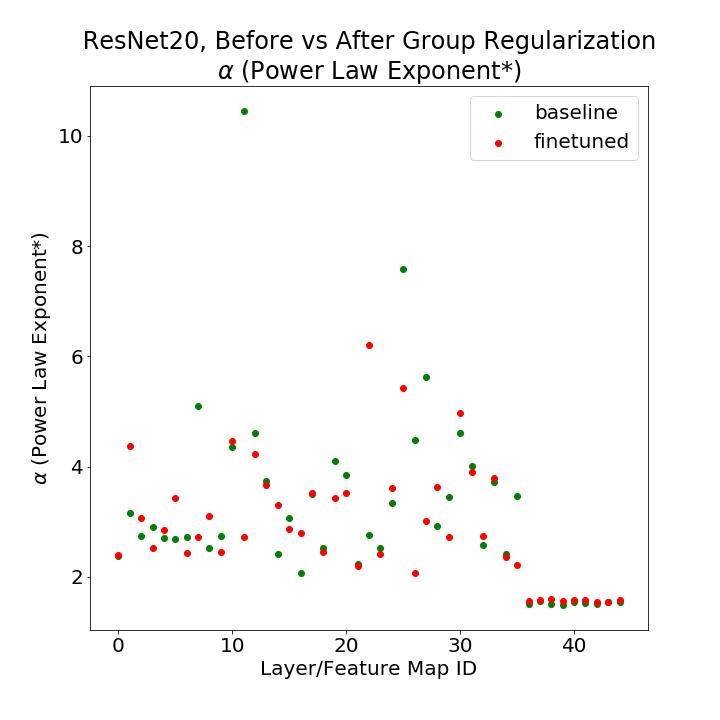
\includegraphics[width=4.9cm]{img/resnet4d_alphas.png}
      \label{fig:resnet204Dalpha}
   }
   \caption{%Correlation Flow.
            ResNet20, distilled with Group Regularization, as implemented in the \texttt{distiller} (4D\_regularized\_5Lremoved) pretrained models.  
            Log Spectral Norm ($\log\lambda_{max}$) and PL exponent ($\alpha$) for individual layers, versus layer id, for both baseline (before distillation, green) and fine-tuned (after distillation, red) pretrained models. 
           }
   \label{fig:resnet204D5L}
\end{figure}


\paragraph{Scale Collapse; or How Distillation May Break Models.}

The similarity between norm-based metrics and PL-based metrics may lead one to wonder whether the Weighted Alpha metric is just a variation of more familiar norm-based metrics.  
Among hundreds of pretrained models, there are ``exceptions that prove the rule,'' and these can be used to show that fitted $\alpha$ values do contain information not captured by norms. 
To illustrate this, we show that some compression/distillation methods \cite{CWZZ17_TR} may actually damage models unexpectedly, by introducing what we call Scale Collapse, where several distilled layers have unexpectedly small Spectral Norms.

Consider ResNet20, trained on CIFAR10, before and after applying the Group Regularization distillation technique, as implemented in the \texttt{distiller} package~\cite{distiller}.
We analyze the pretrained 4D\_regularized\_5Lremoved baseline and fine-tuned models. 
The reported baseline test accuracies (Top1$=91.45$ and Top5$=99.75$) are better than the reported fine-tuned test accuracies (Top1$=91.02$ and Top5$=99.67$).  
Because the baseline accuracy is greater,  the previous results on ResNet (Table~\ref{table:cv-models} and Figure~\ref{fig:cv2-accuracy}) suggest that the baseline Spectral Norms should be smaller on average than the fine-tuned ones.
The opposite is observed.
Figure~\ref{fig:resnet204D5L} presents the Spectral Norm (here denoted $\log\lambda_{max}$) and PL exponent ($\alpha$) for each individual layer weight matrix $\mathbf{W}$.
On the other hand, the $\alpha$ values (in Figure~\ref{fig:resnet204Dalpha}) do not differ systematically between the baseline and fine-tuned models.
Also (not shown, but as predicted by HT-SR Theory, the basis of $\hat{\alpha}$), the average (unweighted) baseline $\alpha$ is smaller than the fine-tuned average.
%
In spite of this, Figure~\ref{fig:resnet204Dalpha} also depicts two very large $\alpha\gg 6$ values for the baseline, but not for the fine-tuned, model.
This suggests the baseline model has at least two over-parameterized/under-trained layers, and that the distillation method does, in fact, improve the fine-tuned model by compressing these layers.

Pretrained models in the \texttt{distiller} package have passed some quality metric, but they are much less well trodden than any of the VGG, ResNet, or DenseNet series.  
The obvious interpretation is that, while norms make good regularizers for a single model, there is no reason a priori to expect them correlate well with test accuracies across different models, and they may not differentiate well-trained versus poorly-trained models.
We do expect, however, the PL $\alpha$ to do so, because it effectively measures the amount of information correlation in the model~\cite{MM18_TR, MM19_HTSR_ICML, MM20_SDM}.
This suggests that the $\alpha$ values will improve, i.e., decrease, over time, as distillation techniques continue to improve.
The reason for the anomalous behavior shown in 
Figure~\ref{fig:resnet204D5L}
is that the \texttt{distiller} Group Regularization technique 
causes the norms of the $\mathbf{W}$ pre-activation maps for two Conv2D layers to increase spuriously.
This is difficult to diagnose by analyzing training/test curves, but it is easy to diagnose with our~approach.


